
%\documentclass[11pts,a4paper,amsmath,amssymb,floatfix]{article}%{report}%{book}
\documentclass[12pts,a4paper,amsmath,amssymb,floatfix]{article}%{report}%{book}
\usepackage{graphicx,wrapfig,pdfpages}% Include figure files
%\usepackage{dcolumn,enumerate}% Align table columns on decimal point
\usepackage{enumerate,enumitem}% Align table columns on decimal point
\usepackage{bm,dpfloat}% bold math
\usepackage[pdftex,bookmarks,colorlinks=true,urlcolor=rltblue,citecolor=blue]{hyperref}
\usepackage{amsfonts,amsmath,amssymb,stmaryrd,indentfirst}
\usepackage{times,psfrag}
\usepackage{natbib}
\usepackage{color}
\usepackage{units}
\usepackage{rotating}
\usepackage{multirow}


\usepackage{pifont}
\usepackage{subfigure}
\usepackage{subeqnarray}
\usepackage{ifthen}

\usepackage{supertabular}
\usepackage{moreverb}
\usepackage{listings}
\usepackage{palatino}
%\usepackage{doi}
\usepackage{longtable}
\usepackage{float}
\usepackage{perpage}
\MakeSorted{figure}
%\usepackage{pdflscape}


%\usepackage{booktabs}
%\newcommand{\ra}[1]{\renewcommand{\arraystretch}{#1}}


\definecolor{rltblue}{rgb}{0,0,0.75}


%\usepackage{natbib}
\usepackage{fancyhdr} %%%%
\pagestyle{fancy}%%%%
% with this we ensure that the chapter and section
% headings are in lowercase
%%%%\renewcommand{\chaptermark}[1]{\markboth{#1}{}}
\renewcommand{\sectionmark}[1]{\markright{\thesection\ #1}}
\fancyhf{} %delete the current section for header and footer
\fancyhead[LE,RO]{\bfseries\thepage}
\fancyhead[LO]{\bfseries\rightmark}
\fancyhead[RE]{\bfseries\leftmark}
\renewcommand{\headrulewidth}{0.5pt}
% make space for the rule
\fancypagestyle{plain}{%
\fancyhead{} %get rid of the headers on plain pages
\renewcommand{\headrulewidth}{0pt} % and the line
}

\def\newblock{\hskip .11em plus .33em minus .07em}
\usepackage{color}

%\usepackage{makeidx}
%\makeindex

\setlength\textwidth      {16.cm}
\setlength\textheight     {22.6cm}
\setlength\oddsidemargin  {-0.3cm}
\setlength\evensidemargin {0.3cm}

\setlength\headheight{14.49998pt} 
\setlength\topmargin{0.0cm}
\setlength\headsep{1.cm}
\setlength\footskip{1.cm}
\setlength\parskip{0pt}
\setlength\parindent{0pt}


%%%
%%% Headers and Footers
\lhead[] {\text{\small{EX3029 -- Chemical Thermodynamics}}} 
\rhead[] {{\text{\small{Tutorial 05}}}}
%\chead[] {\text{\small{Session 2012/13}}} 
\lfoot[]{Dr Jeff Gomes}
%\cfoot[\thepage]{\thepage}
\rfoot[\text{\small{\thepage}}]{\thepage}
\renewcommand{\headrulewidth}{0.8pt}


%%%
%%% space between lines
%%%
\renewcommand{\baselinestretch}{1.5}

\newenvironment{VarDescription}[1]%
  {\begin{list}{}{\renewcommand{\makelabel}[1]{\textbf{##1:}\hfil}%
    \settowidth{\labelwidth}{\textbf{#1:}}%
    \setlength{\leftmargin}{\labelwidth}\addtolength{\leftmargin}{\labelsep}}}%
  {\end{list}}

%%%%%%%%%%%%%%%%%%%%%%%%%%%%%%%%%%%%%%%%%%%
%%%%%%                              %%%%%%%
%%%%%%      NOTATION SECTION        %%%%%%%
%%%%%%                              %%%%%%%
%%%%%%%%%%%%%%%%%%%%%%%%%%%%%%%%%%%%%%%%%%%

% Text abbreviations.
\newcommand{\ie}{{\em{i.e., }}}
\newcommand{\eg}{{\em{e.g., }}}
\newcommand{\cf}{{\em{cf., }}}
\newcommand{\wrt}{with respect to}
\newcommand{\lhs}{left hand side}
\newcommand{\rhs}{right hand side}
% Commands definining mathematical notation.

% This is for quantities which are physically vectors.
\renewcommand{\vec}[1]{{\mbox{\boldmath$#1$}}}
% Physical rank 2 tensors
\newcommand{\tensor}[1]{\overline{\overline{#1}}}
% This is for vectors formed of the value of a quantity at each node.
\newcommand{\dvec}[1]{\underline{#1}}
% This is for matrices in the discrete system.
\newcommand{\mat}[1]{\mathrm{#1}}


\DeclareMathOperator{\sgn}{sgn}
\newtheorem{thm}{Theorem}[section]
\newtheorem{lemma}[thm]{Lemma}

%\newcommand\qed{\hfill\mbox{$\Box$}}
\newcommand{\re}{{\mathrm{I}\hspace{-0.2em}\mathrm{R}}}
\newcommand{\inner}[2]{\langle#1,#2\rangle}
\renewcommand\leq{\leqslant}
\renewcommand\geq{\geqslant}
\renewcommand\le{\leqslant}
\renewcommand\ge{\geqslant}
\renewcommand\epsilon{\varepsilon}
\newcommand\eps{\varepsilon}
\renewcommand\phi{\varphi}
\newcommand{\bmF}{\vec{F}}
\newcommand{\bmphi}{\vec{\phi}}
\newcommand{\bmn}{\vec{n}}
\newcommand{\bmns}{{\textrm{\scriptsize{\boldmath $n$}}}}
\newcommand{\bmi}{\vec{i}}
\newcommand{\bmj}{\vec{j}}
\newcommand{\bmk}{\vec{k}}
\newcommand{\bmx}{\vec{x}}
\newcommand{\bmu}{\vec{u}}
\newcommand{\bmv}{\vec{v}}
\newcommand{\bmr}{\vec{r}}
\newcommand{\bma}{\vec{a}}
\newcommand{\bmg}{\vec{g}}
\newcommand{\bmU}{\vec{U}}
\newcommand{\bmI}{\vec{I}}
\newcommand{\bmq}{\vec{q}}
\newcommand{\bmT}{\vec{T}}
\newcommand{\bmM}{\vec{M}}
\newcommand{\bmtau}{\vec{\tau}}
\newcommand{\bmOmega}{\vec{\Omega}}
\newcommand{\pp}{\partial}
\newcommand{\kaptens}{\tensor{\kappa}}
\newcommand{\tautens}{\tensor{\tau}}
\newcommand{\sigtens}{\tensor{\sigma}}
\newcommand{\etens}{\tensor{\dot\epsilon}}
\newcommand{\ktens}{\tensor{k}}
\newcommand{\half}{{\textstyle \frac{1}{2}}}
\newcommand{\tote}{E}
\newcommand{\inte}{e}
\newcommand{\strt}{\dot\epsilon}
\newcommand{\modu}{|\bmu|}
% Derivatives
\renewcommand{\d}{\mathrm{d}}
\newcommand{\D}{\mathrm{D}}
\newcommand{\ddx}[2][x]{\frac{\d#2}{\d#1}}
\newcommand{\ddxx}[2][x]{\frac{\d^2#2}{\d#1^2}}
\newcommand{\ddt}[2][t]{\frac{\d#2}{\d#1}}
\newcommand{\ddtt}[2][t]{\frac{\d^2#2}{\d#1^2}}
\newcommand{\ppx}[2][x]{\frac{\partial#2}{\partial#1}}
\newcommand{\ppxx}[2][x]{\frac{\partial^2#2}{\partial#1^2}}
\newcommand{\ppt}[2][t]{\frac{\partial#2}{\partial#1}}
\newcommand{\pptt}[2][t]{\frac{\partial^2#2}{\partial#1^2}}
\newcommand{\DDx}[2][x]{\frac{\D#2}{\D#1}}
\newcommand{\DDxx}[2][x]{\frac{\D^2#2}{\D#1^2}}
\newcommand{\DDt}[2][t]{\frac{\D#2}{\D#1}}
\newcommand{\DDtt}[2][t]{\frac{\D^2#2}{\D#1^2}}
% Norms
\newcommand{\Ltwo}{\ensuremath{L_2} }
% Basis functions
\newcommand{\Qone}{\ensuremath{Q_1} }
\newcommand{\Qtwo}{\ensuremath{Q_2} }
\newcommand{\Qthree}{\ensuremath{Q_3} }
\newcommand{\QN}{\ensuremath{Q_N} }
\newcommand{\Pzero}{\ensuremath{P_0} }
\newcommand{\Pone}{\ensuremath{P_1} }
\newcommand{\Ptwo}{\ensuremath{P_2} }
\newcommand{\Pthree}{\ensuremath{P_3} }
\newcommand{\PN}{\ensuremath{P_N} }
\newcommand{\Poo}{\ensuremath{P_1P_1} }
\newcommand{\PoDGPt}{\ensuremath{P_{-1}P_2} }

\newcommand{\metric}{\tensor{M}}
\newcommand{\configureflag}[1]{\texttt{#1}}

% Units
\newcommand{\m}[1][]{\unit[#1]{m}}
\newcommand{\km}[1][]{\unit[#1]{km}}
\newcommand{\s}[1][]{\unit[#1]{s}}
\newcommand{\invs}[1][]{\unit[#1]{s}\ensuremath{^{-1}}}
\newcommand{\ms}[1][]{\unit[#1]{m\ensuremath{\,}s\ensuremath{^{-1}}}}
\newcommand{\mss}[1][]{\unit[#1]{m\ensuremath{\,}s\ensuremath{^{-2}}}}
\newcommand{\K}[1][]{\unit[#1]{K}}
\newcommand{\PSU}[1][]{\unit[#1]{PSU}}
\newcommand{\Pa}[1][]{\unit[#1]{Pa}}
\newcommand{\kg}[1][]{\unit[#1]{kg}}
\newcommand{\rads}[1][]{\unit[#1]{rad\ensuremath{\,}s\ensuremath{^{-1}}}}
\newcommand{\kgmm}[1][]{\unit[#1]{kg\ensuremath{\,}m\ensuremath{^{-2}}}}
\newcommand{\kgmmm}[1][]{\unit[#1]{kg\ensuremath{\,}m\ensuremath{^{-3}}}}
\newcommand{\Nmm}[1][]{\unit[#1]{N\ensuremath{\,}m\ensuremath{^{-2}}}}

% Dimensionless numbers
\newcommand{\dimensionless}[1]{\mathrm{#1}}
\renewcommand{\Re}{\dimensionless{Re}}
\newcommand{\Ro}{\dimensionless{Ro}}
\newcommand{\Fr}{\dimensionless{Fr}}
\newcommand{\Bu}{\dimensionless{Bu}}
\newcommand{\Ri}{\dimensionless{Ri}}
\renewcommand{\Pr}{\dimensionless{Pr}}
\newcommand{\Pe}{\dimensionless{Pe}}
\newcommand{\Ek}{\dimensionless{Ek}}
\newcommand{\Gr}{\dimensionless{Gr}}
\newcommand{\Ra}{\dimensionless{Ra}}
\newcommand{\Sh}{\dimensionless{Sh}}
\newcommand{\Sc}{\dimensionless{Sc}}


% Journals
\newcommand{\IJHMT}{{\it International Journal of Heat and Mass Transfer}}
\newcommand{\NED}{{\it Nuclear Engineering and Design}}
\newcommand{\ICHMT}{{\it International Communications in Heat and Mass Transfer}}
\newcommand{\NET}{{\it Nuclear Engineering and Technology}}
\newcommand{\HT}{{\it Heat Transfer}}   
\newcommand{\IJHT}{{\it International Journal for Heat Transfer}}

\newcommand{\frc}{\displaystyle\frac}

\newlist{ExList}{enumerate}{1}
\setlist[ExList,1]{label={\bf Example 1.} {\bf \arabic*}}

\newlist{ProbList}{enumerate}{1}
\setlist[ProbList,1]{label={\bf Problem 1.} {\bf \arabic*}}

%%%%%%%%%%%%%%%%%%%%%%%%%%%%%%%%%%%%%%%%%%%
%%%%%%                              %%%%%%%
%%%%%% END OF THE NOTATION SECTION  %%%%%%%
%%%%%%                              %%%%%%%
%%%%%%%%%%%%%%%%%%%%%%%%%%%%%%%%%%%%%%%%%%%


% Cause numbering of subsubsections. 
%\setcounter{secnumdepth}{8}
%\setcounter{tocdepth}{8}

\setcounter{secnumdepth}{4}%
\setcounter{tocdepth}{4}%


\begin{document}



\begin{enumerate}[label=\bfseries Problem \arabic*:]

%%%
%%% Johannes T06E01
%%%
\item\label{T06E01}For a lab experiment an amount of 2 litres of an antifreeze solution is required. The solution should consist of 30 mol$\%$ methanol in water. Determine the volumes of pure methanol and pure water at 25$^{\circ}$C that must be mixed to yield the 2 litres of solution. Partial molar volumes $\left(\overline{V}_{i}\right)$ for methanol and water in 30 mol$\%$ methanol solution and their pure-species molar volumes $\left(V_{i}\right)$, both at 25$^{\circ}$C, are,
\begin{center}
\begin{tabular}{l l c l} 
     Methanol (1): & $\overline{V}_{1}$=38.632 $\frac{\text{cm}^{3}}{\text{mol}}$ & \hspace{1cm} & $V_{1}$=40.727 $\frac{\text{cm}^{3}}{\text{mol}}$ \\
     Water (2):    & $\overline{V}_{2}$=17.765 $\frac{\text{cm}^{3}}{\text{mol}}$ & \hspace{1cm} & $V_{2}$=18.068 $\frac{\text{cm}^{3}}{\text{mol}}$ 
\end{tabular}
\end{center} 

What would be the volume if an ideal solution were formed?  

%%%
%%% Johannes T0602
%%%
\item\label{T0602} What is the change in entropy when 700 litres of CO$_{2}$ and 300 litres of N$_{2}$, each at 1 bar and 25$^{\circ}$C blend to form a gas mixture at the same conditions? Assume ideal gas behaviour and that {\it mole fraction = volume fraction}.

%%%
%%% Johannes T0701
%%%
\item\label{T0701} The following expressions have been proposed for the partial molar properties of a particular binary mixture:
\begin{displaymath}
\overline{M}_{1} = M_{1} + A x_{2} \hspace{2cm} \overline{M}_{2} = M_{2} + A x_{1} 
\end{displaymath}
Here, parameter $A$ is a constant. Can these expressions possibly be correct? Explain.

%%%
%%% Johannes T0702
%%%
\item\label{T0702} The volume change of mixing $\left(\text{in cm}^{3}\text{.mol}^{-1}\right)$ for the system ethanol (1) and methy-butyl ether (2) at 25$^{\circ}$C is given by the equation
\begin{displaymath}
\Delta V_{\text{mix}} = x_{1} x_{2}\left[-1.026+0.220\left(x_{1}-x_{2}\right)\right]
\end{displaymath} 
Given the molar volume of pure species, V$_{1}$=58.63 cm$^{3}$.mol$^{-1}$ and V$_{2}$=118.46 cm$^{3}$.mol$^{-1}$, what volume of mixture is formed when 750 cm$^{3}$ of pure species 1 is mixed with 1500 cm$^{3}$ of species 2 at 25$^{\circ}$C? What would be the volume if an ideal solution were formed?


%%%
%%% Sandler Examples 9.3.2-3 (pgs 414-416)
%%%
%\item\label{Ex1} During an experiment, a student determined that the Gibbs energy of a binary mixture was of the form,
%\begin{displaymath}
%\overline{G}^{\text{mix}}\left(T,P,y\right) = \sum\limits_{i=1}^{2}y_{i}\overline{G}_{i}\left(T,P\right) + RT\sum\limits_{i=1}^{2}y_{i}\ln y_{i} + a y_{1} y_{2}
%\end{displaymath}
%where $a$ is a constant. 
%\begin{enumerate}
%\item Determine whether this mixture is an ideal gas mixture.
%\item Develop an expression for the activity coefficients and species fugacities using the Gibbs energy function, $\overline{G}^{\text{mix}}$.
%\end{enumerate}

%%%
%%% SM &VN 11.13
%%%
\item\label{Ex2} The molar volume $\left(\text{in cm}^{3}\text{.mol}^{-1}\right)$ of a binary liquid mixture at $T$ and $P$ is given by:
\begin{displaymath}
V = 120 x_{1} + 70 x_{2} + \left( 15x_{1} + 8x_{2}\right)x_{1}x_{2} 
\end{displaymath}
\begin{enumerate}
\item\label{first} Find expressions for the partial molar volumes of species 1 and 2 at $T$ and $P$.
\item Show that when these expressions are combined in accord with $M=\sum\limits_{i}x_{i}\overline{M}_{i}$, the given equation for $V$ is recovered;
\item Show that these expressions satisfy the Gibbs-Duhem equation, $\sum\limits_{i}x_{i}d\overline{M}_{i}=0$;
\item Show that 
   \begin{displaymath}
        \left(\frc{d\overline{V}_{1}}{dx_{1}}\right)_{x_{1}=1} = \left(\frc{d\overline{V}_{2}}{dx_{1}}\right)_{x_{1}=0} = 0
   \end{displaymath}
 \item Plot values of $V$, $\overline{V}_{1}$ and $\overline{V}_{2}$ calculated by the given equation for $V$ and by the equations developed in (a) {\it vs} $x_{1}$. Label points $\overline{V}_{1}^{\infty}$ and $\overline{V}_{2}^{\infty}$ and show their values.
\end{enumerate} 

%%%
%%% 
%%%
%\item\label{P6} Two litres of an anti-freezing solution is needed for a cooling process. The solution is prepared by mixing 30$\%$-mol of methanol in water. What are the volumes of pure methanol and water at 25$^{\circ}$C necessary to prepare solution? Partial molar volumes $\left(\overline{V}\right)$ for methanol and water in a 30$\%$-mol of methanol solution and their pure species molar volumes $\left(V\right)$, both at 25$^{\circ}$C are:
%       \begin{center}
%          \begin{tabular}{ l l l }
%                             & $\overline{V}_{i} \left(\text{cm}^{3}.\text{mol}^{-1}\right)$ & $V_{i} \left(\text{cm}^{3}.\text{mol}^{-1}\right)$ \\
%               Methanol (1)  & 38.6320                                                     & 40.7270  \\
%               Water (2)     & 17.7650                                                     & 18.0680 
%          \end{tabular}
%       \end{center}
%%%
%%% 
%%%
\item\label{P7} In generating expressions from $G^{E}/RT$ from VLE data, a convenient approach is to plot values of $G^{E}/\left(x_{1}x_{2}RT\right)$ {\it vs} $x_{1}$ and fitting results with an appropriate function. Consider if such data were fit by the expression,
   \begin{displaymath}
       \frc{G^{E}}{x_{1}x_{2} R T} = A + B x_{1}^{2}.
   \end{displaymath}
         From the expression $G^{E}/\left(x_{1}x_{2}RT\right)$, provide equations for the activity coefficient, $\ln{\gamma_{i}}$, as a function of $A$, $B$ and $x_{1}$, given
       \begin{displaymath}
               \ln{\gamma_{i}} = \frc{\overline{G}_{i}^{E}}{RT}.
       \end{displaymath} 

\end{enumerate} 

%{
%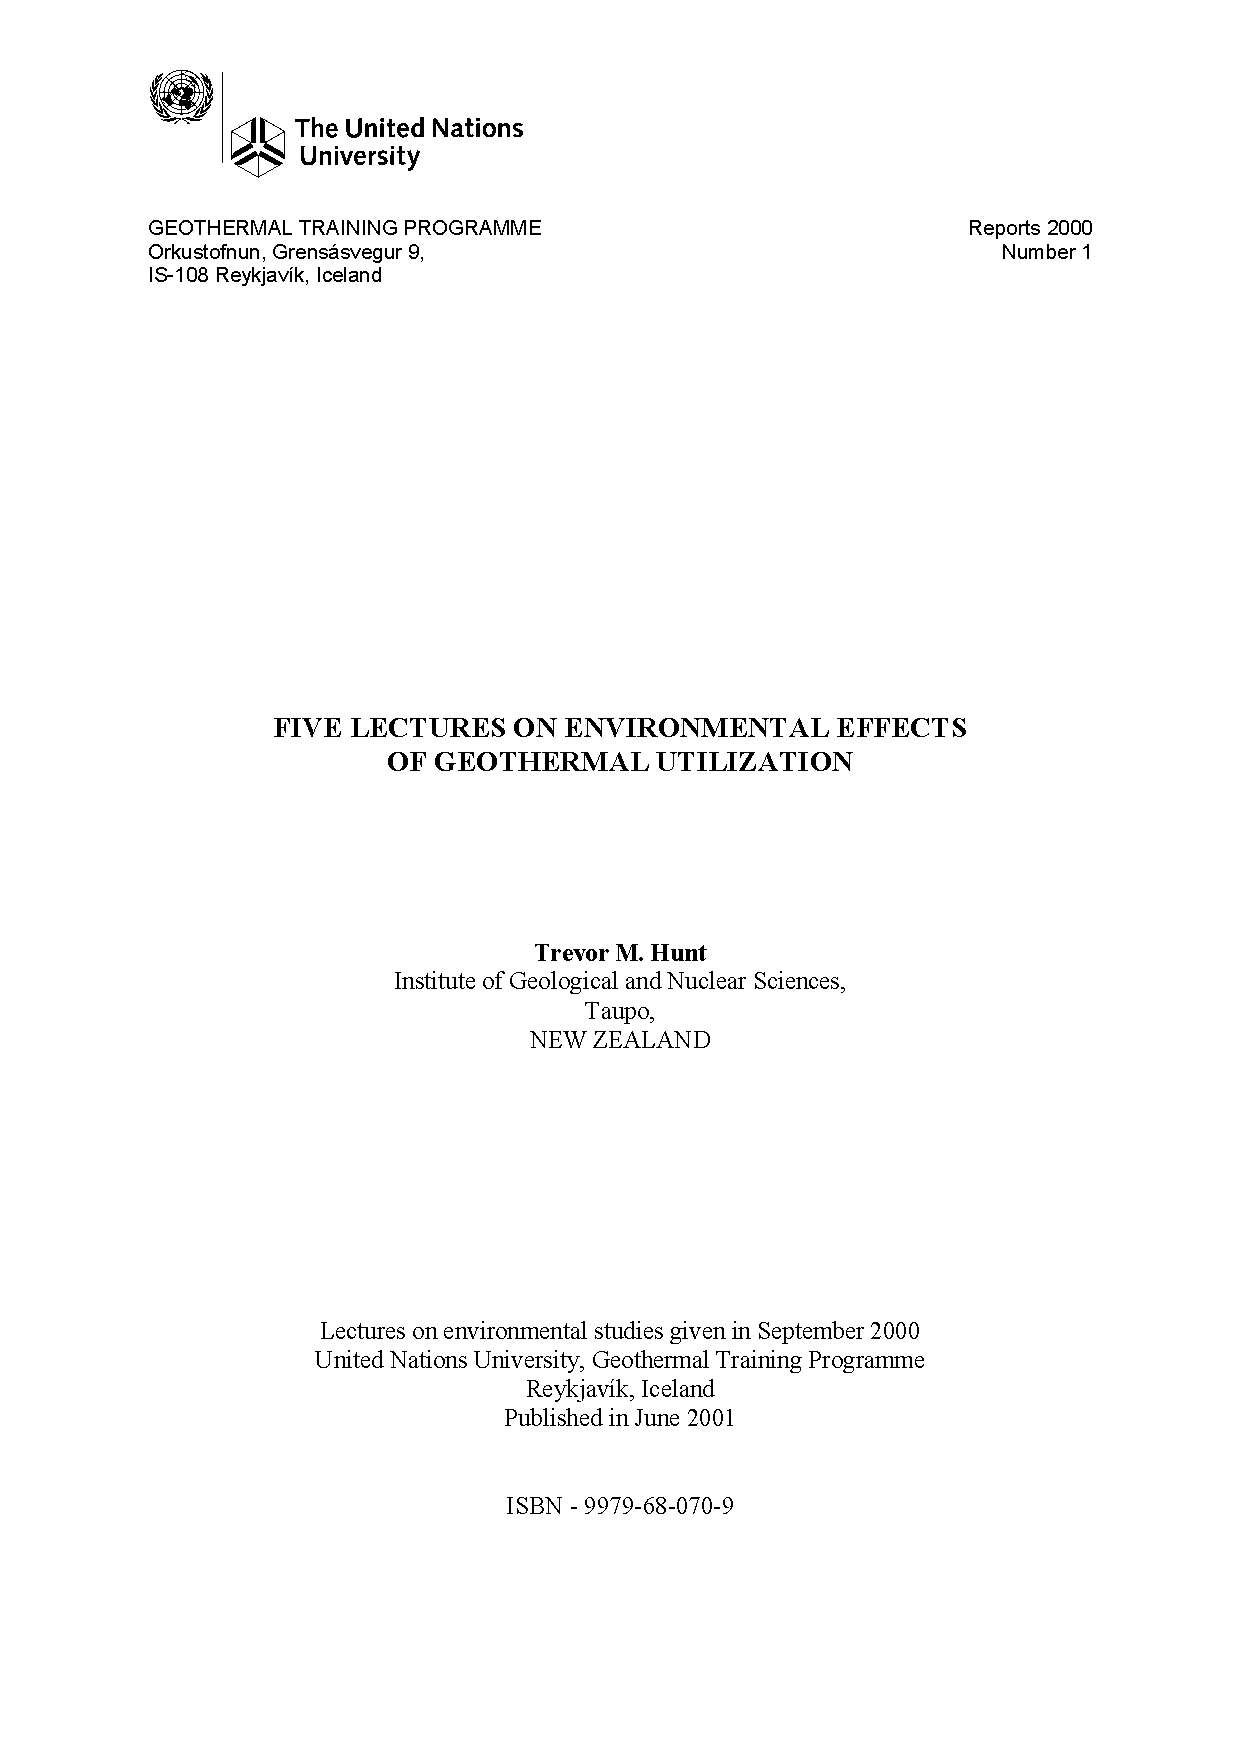
\includepdf[pages=-,fitpaper, angle=0]{./HuntSelect.pdf}
%}

\end{document}
